\chapter{Выполнение работы}

\section{Расчётные соотношения}

В списке ниже в скобках указаны идентификаторы соответствующих величин, рассчитываемые в программе.

\begin{itemize}[$\bullet$]
	\item Максимальное значение выборки $\overrightarrow{x_n}$ ~~~(\texttt{M\_max})

	\begin{equation}
		M_{max} = x_{(n)}
	\end{equation}

	\item Минимальное значение выборки ~~~(\texttt{M\_min})
	
	\begin{equation}
		M_{min} = x_{(1)}
	\end{equation}

	\item Размах выборки ~~~(\texttt{R})
	
	\begin{equation}
		R = x_{(n)} - x_{(1)}
	\end{equation}

	\item Оценка математического ожидания ~~~(\texttt{mu\_hat})
	
	\begin{equation}
		\hat\mu(\overrightarrow{x_n}) = \frac{1}{n} \sum_{i=1}^{n} x_i
	\end{equation}

	\item Исправленная ценка дисперсии ~~~(\texttt{S\_2})
	
	\begin{equation}
		S^2(\overrightarrow{x_n}) = \frac{1}{n-1} \sum_{i=1}^{n} (x_i - \overline{x})^2
	\end{equation}

	\item Количество интервалов в интервальном статистическом ряду ~~~(\texttt{m})
	
	\begin{equation}
		m = \lfloor \log_2 n \rfloor + 2
	\end{equation}

\end{itemize}

\clearpage

\section{Определение эмпирической плотности и гистограммы}

\textbf{Определение}: интервальным статистическим рядом отвечающим выборке $\overrightarrow{x}$ называется таблица вида

\begin{table}
	\centering
	\begin{tabular}{|c|c|c|c|}
		\hline
		$J_1$ & $J_2$ & $\dots$ & $J_m$ \\
		\hline
		$n_1$ & $n_2$ & $\dots$ & $n_m$ \\
		\hline
	\end{tabular}
\end{table}

в которой

\begin{itemize}[]
	\item $J_i = [x_{(1)} + (i - 1) \Delta;~x_{(1)} + i \Delta),~~~i = \overline{1,m-1}$
	
	\item $J_m = [x_{(1)} + (m - 1) \Delta;~x_{(n)}]$
	
	\item $\displaystyle \Delta = \frac{|J|}{m} = \frac{x_{(n)} - x_{(1)}}{m}$
	
	\item $n_i$ -- число элементов выборки $\overrightarrow{x}$ попавших в $J_i$.
	
\end{itemize}

\textbf{Определение}: эмпирической плотностью распределения, соответствующей выборке $\overrightarrow{x}$, называется функция

\begin{equation}
	f_n(x) = \left\{\begin{array}{ll}
		{\displaystyle \frac{n_i}{n \Delta},} & x \in J_i \\
		0, & \textit{иначе}
	\end{array}\right.
\end{equation}

\textbf{Определение}: график эмпирической функции плотности называется гистограммой.

\section{Определение эмпирической функции распределения}

Пусть $\overrightarrow{x} = (x_1, x_2, \dots, x_n)$ -- выборка из генеральной совокупности $X$.

Обозначим $n(t, \overrightarrow{x})$ -- число компонент вектора $\overrightarrow{x}$, которые меньше, чем $t$.

\textbf{Определение}: эмпирической функцией распределения построенной по выборке $\overrightarrow{x}$ называется функция

\begin{equation}
	F_n: \mathbb{R} \rightarrow \mathbb{R},
\end{equation}

определённая правилом

\begin{equation}
	F_n(t) = \frac{n(t, \overrightarrow{x})}{n}.
\end{equation}

\clearpage

\section{Результаты работы}

\begin{table}
	\centering
	\begin{tabular}{|c|c|}
		\hline
		\textbf{~~Величина~~} & \textbf{~~Значение~~} \\
		\hline
		\texttt{N} & \texttt{120} \\
		\texttt{M\_min} & \texttt{-2.77} \\
		\texttt{M\_max} & \texttt{2.92} \\
		\texttt{R} & \texttt{5.69} \\
		\texttt{mu\_hat} & \texttt{0.2322} \\
		\texttt{S\_2} & \texttt{1.0406} \\
		\texttt{m} & \texttt{8} \\
		\hline
	\end{tabular}
	\caption{Результаты вычислений параметров выборки}
\end{table}

\begin{figure}
	\centering	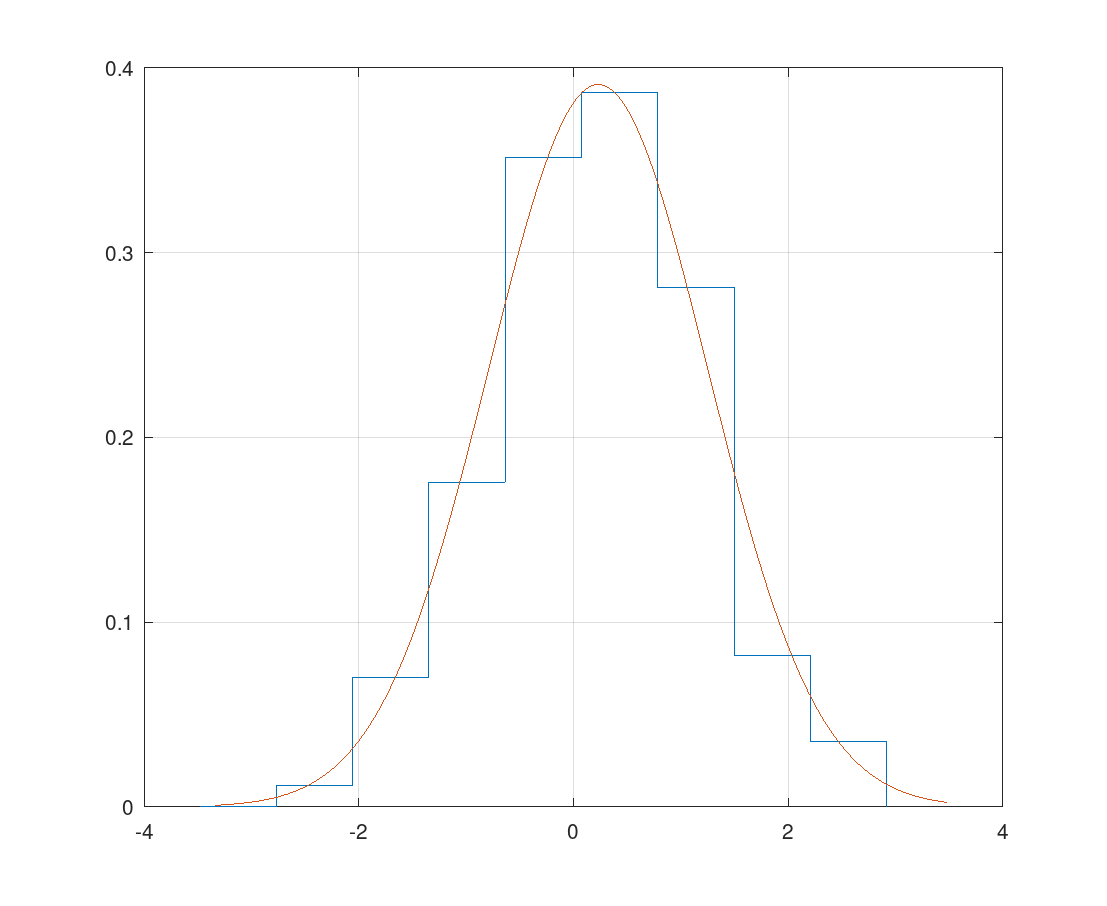
\includegraphics[width=0.8\linewidth]{img/screenshot002}
	\caption{Гистограмма и график функции плотности распределения вероятностей нормальной случайной величины $Y\sim\mathbb{N}(\hat{\mu}, S^2)$}
	\label{fig:screenshot002}
\end{figure}

\begin{figure}
	\centering
	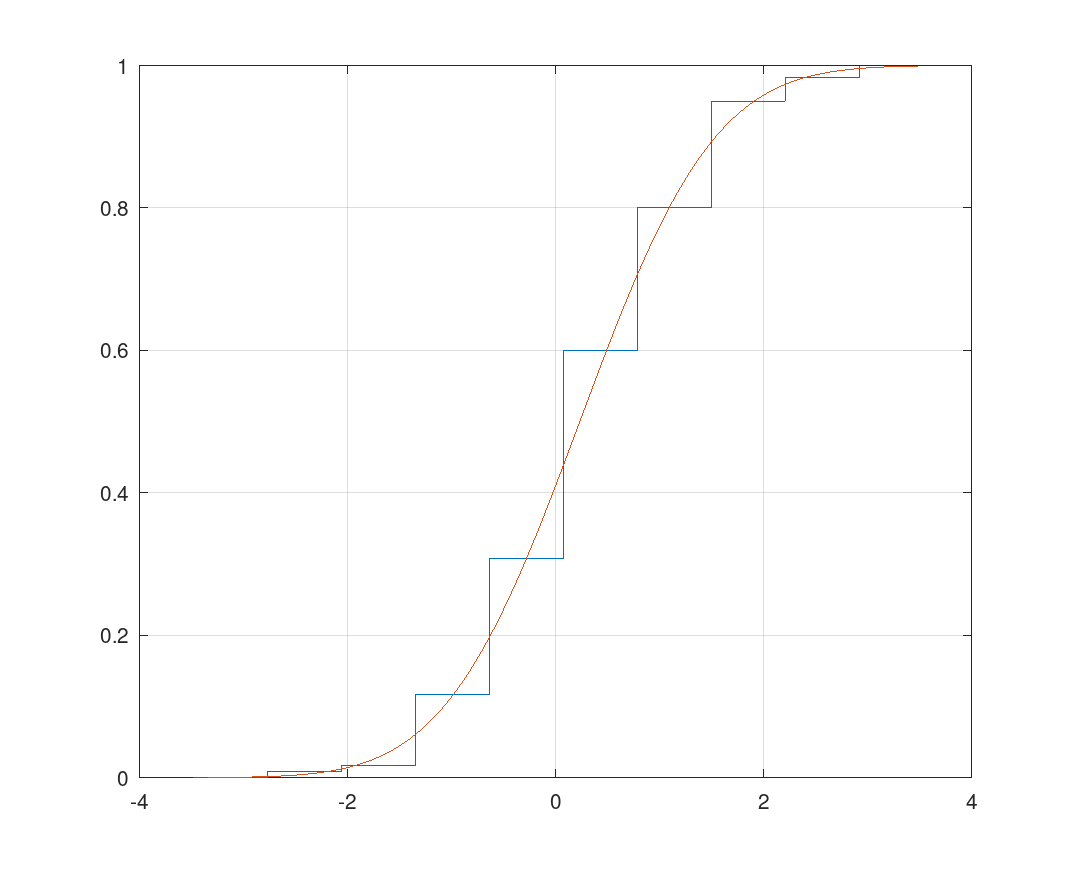
\includegraphics[width=\linewidth]{img/screenshot003}
	\caption{График эмпирической функции распределения и функции распределения нормальной случайной величины $Y\sim\mathbb{N}(\hat{\mu}, S^2)$}
	\label{fig:screenshot003}
\end{figure}

\clearpage

\section{Текст программы}

\begin{lstlisting}
#!/bin/octave -qf

pkg load statistics

X = [-0.45, -0.33, 2.92, -1.25, -1.20, 0.05, -0.53, -0.19, 1.49, 0.67, 0.22, 1.23, 0.50, -0.92, 0.90, -1.52, -0.15, -1.24, -0.47, -0.45, 0.18, -0.05, 1.58, 1.74, 2.37, -0.24, -1.34, 1.05, 1.28, 1.37, 1.18, 0.22, 0.11, 0.28, -0.64, -0.39, -1.77, -1.61, 0.47, 0.77, -0.27, -1.19, -0.25, 1.04, -0.16, 0.42, 0.29, 0.10, 1.04, 0.43, -0.67, 0.41, -0.62, -1.49, 1.46, -2.77, 2.09, 0.88, -0.36, -0.71, -0.62, 1.34, -0.78, -0.15, 2.69, 0.92, 1.68, -0.12, 0.34, 0.74, 1.72, 1.24, 0.23, 0.76, 0.87, -1.52, 0.63, -0.56, 0.83, 0.31, -0.18, 0.99, -1.01, 0.58, 1.21, -1.51, 0.65, 0.35, -0.37, -0.50, -0.73, 0.63, 0.33, 1.56, -0.98, 0.85, 0.56, -1.07, 1.47, 1.44, 1.91, 0.24, 1.34, 0.99, 1.27, 0.11, 0.22, -0.25, 0.35, -0.03, -0.56, -0.79, 2.41, -0.45, -0.44, 0.07, 0.64, 0.69, 0.10, -0.28];

N = length(X)
[M_min, M_max] = bounds(X)          # Минимальное и максимальное значения выборки
R = range(X)                        # Размах выборки

mu_hat = sum(X) / N                 # Среднее наблюдённое значение
S_2 = sum((X - mu_hat).^2) / (N-1)  # Оценка дисперсии

m = floor(log2(N)) + 2              # Количество интервалов
intv_delta = R / m                  # Размер интервала

intv = zeros(2, m);                 # Интервалы
n = zeros(1, m);                    # Частости значений в интервалах 

for k = 1:m
	intv(1, k) = X_min + (k - 1) * intv_delta;
	intv(2, k) = X_min + k * intv_delta;
	n(1, k) = sum(intv(1, k) <= X & X < intv(2, k)) / intv_delta / N;
endfor;

X_norm = linspace(M_min, M_max, 200);
Y_norm = 1 / (2 * sqrt(S_2)) * exp(-(X_norm - mu_hat) .^ 2);

stairs(intv(1, 1:m), n);            # Вывод ступенчатого графика функции плотности
hold on
plot(X_norm, Y_norm);               # Вывод графика функции плотности
hold off
pause;

n = cumsum(n) * intv_delta;
Y_norm = stdnormal_cdf((X_norm - mu_hat) / sqrt(S_2));
\end{lstlisting}

\clearpage

\begin{lstlisting}[firstnumber=37]
stairs(intv(1, 1:m), n);            # Вывод эмпирической функции распределения
hold on
plot(X_norm, Y_norm);               # Вывод функции распределения
hold off
pause;
\end{lstlisting}

%\section{Выборка для заданий 1-2}

%X = (-0.45, -0.33, 2.92, -1.25, -1.20, 0.05, -0.53, -0.19, 1.49, 0.67, 0.22, 1.23, 0.50, -0.92, 0.90, -1.52, -0.15, -1.24, -0.47, -0.45, 0.18, -0.05, 1.58, 1.74, 2.37, -0.24, -1.34, 1.05, 1.28, 1.37, 1.18, 0.22, 0.11, 0.28, -0.64, -0.39, -1.77, -1.61, 0.47, 0.77, -0.27, -1.19, -0.25, 1.04, -0.16, 0.42, 0.29, 0.10, 1.04, 0.43, -0.67, 0.41, -0.62, -1.49, 1.46, -2.77, 2.09, 0.88, -0.36, -0.71, -0.62, 1.34, -0.78, -0.15, 2.69, 0.92, 1.68, -0.12, 0.34, 0.74, 1.72, 1.24, 0.23, 0.76, 0.87, -1.52, 0.63, -0.56, 0.83, 0.31, -0.18, 0.99, -1.01, 0.58, 1.21, -1.51, 0.65, 0.35, -0.37, -0.50, -0.73, 0.63, 0.33, 1.56, -0.98, 0.85, 0.56, -1.07, 1.47, 1.44, 1.91, 0.24, 1.34, 0.99, 1.27, 0.11, 0.22, -0.25, 0.35, -0.03, -0.56, -0.79, 2.41, -0.45, -0.44, 0.07, 0.64, 0.69, 0.10, -0.28)

%\section{Выборки для задания 3}

%T = (-5.00, -4.80, -4.60, -4.40, -4.20, -4.00, -3.80, -3.60, -3.40, -3.20, -3.00, -2.80, -2.60, -2.40, -2.20, -2.00, -1.80, -1.60, -1.40, -1.20, -1.00, -0.80, -0.60, -0.40, -0.20, 0.00, 0.20, 0.40, 0.60, 0.80, 1.00, 1.20, 1.40, 1.60, 1.80, 2.00, 2.20, 2.40, 2.60, 2.80, 3.00, 3.20, 3.40, 3.60, 3.80, 4.00, 4.20, 4.40, 4.60, 4.80, 5.00, 5.20, 5.40, 5.60, 5.80, 6.00, 6.20, 6.40, 6.60, 6.80, 7.00)

%Y = (168.04, 134.84, 151.80, 122.02, 124.47, 99.41, 83.67, 79.85, 67.28, 49.34, 38.70, 37.60, 56.74, 39.18, 14.90, 18.16, 5.57, 20.01, 7.47, -0.83, -4.27, 6.99, -5.98, 0.06, 5.12, 4.25, 11.96, -3.26, 11.99, 1.46, 6.77, 7.04, 20.57, 17.30, 11.79, 27.22, 41.66, 37.30, 54.07, 60.48, 69.80, 99.22, 92.88, 90.04, 115.74, 109.33, 124.73, 155.13, 151.89, 177.92, 188.00, 193.02, 215.24, 227.41, 250.07, 248.79, 286.57, 294.65, 326.11, 341.49, 351.17)
